\documentclass[
	12pt,
	BCOR=5mm,
	DIV=12,
	headinclude=on,
	footinclude=off,
	parskip=half,
	bibliography=totoc,
	listof=entryprefix,
	toc=listof,
	pointlessnumbers,
    plainfootsepline]{scrreprt}
    
% !TEX root =  master.tex

%		LANGUAGE SETTINGS AND FONT ENCODING 
%
\usepackage[ngerman]{babel} 	% German language
\usepackage[utf8]{inputenc}
\usepackage[german=quotes]{csquotes} 	% correct quotes using \enquote{}
\usepackage[T1]{fontenc}
\usepackage{lipsum}
\usepackage[hidelinks=true]{hyperref}
\usepackage{amssymb} % Math symbols
\usepackage[onehalfspacing]{setspace} % Zeileabstand
\usepackage{ gensymb }
\usepackage{ftnxtra}
\usepackage{rotating}
%\usepackage[english]{babel}   % For english language
%\usepackage{csquotes} 	% Richtiges Setzen der Anführungszeichen mit \enquote{}

% 		HYPERREF
%
% \usepackage[
% 	hidelinks=true % keine roten Markierungen bei Links
% ]{hyperref}


% Zwei eigene Befehle zum Setzen von Autor und Titel. Ausserdem werden die PDF-Informationen richtig gesetzt.
\newcommand{\TitelDerArbeit}[1]{\def\DerTitelDerArbeit{#1}\hypersetup{pdftitle={#1}}}
\newcommand{\AutorDerArbeit}[1]{\def\DerAutorDerArbeit{#1}\hypersetup{pdfauthor={#1}}}
\newcommand{\Firma}[1]{\def\DerNameDerFirma{#1}}
\newcommand{\Kurs}[1]{\def\DieKursbezeichnung{#1}}


% Correct superscripts 
\usepackage{fnpct}




%		CALCULATIONS
%
\usepackage{calc} % Used for extra space below footsepline



%		BIBLIOGRAPHY SETTINGS
%

% Uncomment the next three lines for author-year-style with footnotes (Chicago)
\usepackage[backend=biber, autocite=footnote, style=authoryear, dashed=false]{biblatex} 	%Use Author-Year-Cites with footnotes
\AdaptNoteOpt\footcite\multfootcite   %will add  separators if footcite is called multiple consecutive times 
\AdaptNoteOpt\autocite\multautocite % will add  separators if autocite is called multiple consecutive times

% Uncomment the next line for IEEE-style 
% \usepackage[backend=biber, autocite=inline, style=ieee]{biblatex} 	% Use IEEE-Style (e.g. [1])

% Uncomment the next line for alphabetic style 
% \usepackage[backend=biber, autocite=inline, style=alphabetic]{biblatex} 	% Use alphabetic style (e.g. [TGK12])

% Uncomment the next two lines vor Harvard-Style 
%\usepackage[backend=biber, style=apa]{biblatex} 	
%\DeclareLanguageMapping{german}{german-apa}


\DefineBibliographyStrings{ngerman}{  %Change u.a. to et al. (german only!)
	andothers = {{et\,al\adddot}},
}

%%% Uncomment the following lines to support hard URL breaks in bibliography 
%\apptocmd{\UrlBreaks}{\do\f\do\m}{}{}
%\setcounter{biburllcpenalty}{9000}% Kleinbuchstaben
%\setcounter{biburlucpenalty}{9000}% Großbuchstaben


\setlength{\bibparsep}{\parskip}		%add some space between biblatex entries in the bibliography
\addbibresource{bibliography.bib}	%Add file bibliography.bib as biblatex resource


%		FOOTNOTES 
%
% Count footnotes over chapters
\usepackage{chngcntr}
\counterwithout{footnote}{chapter}


%	ACRONYMS
%%%
%%% WICHTIG: Installieren Sie das neueste Acronyms-Paket!!!
%%%
\makeatletter
\usepackage[printonlyused]{acronym}
\@ifpackagelater{acronym}{2015/03/20}
  {%
    \renewcommand*{\aclabelfont}[1]{\textbf{\textsf{\acsfont{#1}}}}
  }%
  {%
  }%
\makeatother

%		LISTINGS
\usepackage{color}
\usepackage{listings}	%Format Listings properly
% Color
\definecolor{Gray}{RGB}{119, 162, 247}
\definecolor{Blue}{RGB}{209, 227, 255}
\definecolor{DarkBlue}{RGB}{38, 58, 209}
\definecolor{Green}{RGB}{184, 255, 222}
\definecolor{Red}{RGB}{255, 206, 184} 
\definecolor{DarkPurple}{rgb}{0.4,0.2,0.6}
\definecolor{GreenCom}{rgb}{0.3,0.5,0.3} 
\definecolor{OrangeString}{RGB}{212, 158, 21}
 
% \makeatletter
% \providecommand\phantomcaption{\caption@refstepcounter\@captype}
% \makeatother

\renewcommand{\lstlistingname}{Quelltext} 
\renewcommand{\lstlistlistingname}{Quelltextverzeichnis}
\lstset{numbers=left,
  numberstyle=\tiny,
  language=Java,
  frame=single,
    captionpos=b,
  basicstyle=\ttfamily\small,
  keywordstyle=\bfseries\color{DarkBlue},
  commentstyle=\itshape\color{GreenCom},
  stringstyle=\color{OrangeString},
  aboveskip=30pt,
  belowskip=30pt,
  breaklines=true
}

%		EXTRA PACKAGES
\usepackage{scrextend}
\usepackage{subfig}
\usepackage{graphicx} % use various graphics formats
\usepackage[german]{varioref} 	% nicer references \vref
\usepackage[font=onehalfspacing]{caption}	%better Captions
\usepackage{booktabs} %nicer Tabs
\usepackage{array}
%\usepackage[T1]{fontenc}
%\usepackage{amssymb}
\usepackage{algcompatible}
\usepackage{mwe}    % loads »blindtext« and »graphicx«
\usepackage{amsmath}
\usepackage{multirow}
% \usepackage{subfig}
% \usepackage{unicode-math}
% \usepackage{algorithmicx}
% \usepackage{algpseudocode}

%\newcolumntype{P}[1]{>{\raggedright\arraybackslash}p{#1}}


		% ALGORITHMS
\usepackage{algorithm}
\usepackage{algpseudocode}
% \usepackage{algorithm,algpseudocode}
\renewcommand{\listalgorithmname}{Algorithmenverzeichnis }
\floatname{algorithm}{Algorithmus}


%		FONT SELECTION: Entweder Latin Modern oder Times / Helvetica
\usepackage{lmodern} %Latin modern font
%\usepackage{mathptmx}  %Helvetica / Times New Roman fonts (2 lines)
%\usepackage[scaled=.92]{helvet} %Helvetica / Times New Roman fonts (2 lines)

%		PAGE HEADER / FOOTER
%	    Warning: There are some redefinitions throughout the master.tex-file!  DON'T CHANGE THESE REDEFINITIONS!
\RequirePackage[automark,headsepline,footsepline]{scrlayer-scrpage}
\pagestyle{scrheadings}
\renewcommand*{\pnumfont}{\upshape\sffamily}
\renewcommand*{\headfont}{\upshape\sffamily}
\renewcommand*{\footfont}{\upshape\sffamily}
\renewcommand{\chaptermarkformat}{}
\RedeclareSectionCommand[beforeskip=0pt]{chapter}
\clearscrheadfoot

\ifoot[\rule{0pt}{\ht\strutbox+\dp\strutbox}DHBW Mannheim]{\rule{0pt}{\ht\strutbox+\dp\strutbox}DHBW Mannheim}
\ofoot[\rule{0pt}{\ht\strutbox+\dp\strutbox}\pagemark]{\rule{0pt}{\ht\strutbox+\dp\strutbox}\pagemark}

\ohead{\headmark}


\begin{document}


\TitelDerArbeit{Planung und Organisation der MOBTS 2022 an der DHBW Mannheim}
\AutorDerArbeit{Tizian Groß, Tristan Emig, Anton Ochel, Benno Grimm, Anna-Lena Richert, Marcel Mertens, Marleen Benner}
\Firma{SAP SE \& Jobrouter}
\Kurs{WWI 18 SE A}

\begin{titlepage}
    
    \begin{minipage}{\textwidth}
        \vspace{5em}
        \begin{center}
            
\includegraphics[width=0.4\textwidth]{img/logo.jpg}
        \end{center}
    \end{minipage}
    \vspace{1em}
    \sffamily

    \begin{center}
        \textsf{\large{}Duale Hochschule Baden-W\"urttemberg\\[1.5mm] Mannheim}\\[2em]
        \textsf{\textbf{\Large{}Seminararbeit}}\\[3mm]
        \textsf{\textbf{\DerTitelDerArbeit}} \\[1.5cm]
        \textsf{\textbf{\Large{}Studiengang Wirtschaftsinformatik}\\[3mm] \textsf{Studienrichtung Software Engineering}}
        
        \vspace{10em}
        %\textsf{\Large{Sperrvermerk}}
    \end{center}
     
    % \begin{center}
    %     \textbf{Tizian Groß} (tizian.gross@mail.com), \textbf{Tristan Emig} (tizian.gross@mail.com) \textbf{Anton Ochel} (tizian.gross@mail.com) \textbf{Benno Grimm} (tizian.gross@mail.com) \textbf{Anna-Lena Richert} (tizian.gross@mail.com) \textbf{Marcel Mertens} (tizian.gross@mail.com) \textbf{Marleen Benner} (tizian.gross@mail.com)
    % \end{center}
    \newpage



    \begin{center}
        \vspace{5em}
        \textbf{Autoren} \\
        \DerAutorDerArbeit
        \vspace{5em}
    \end{center}
       
    
    
        \begin{minipage}{\textwidth}
    
            \begin{tabbing}
                
                Bearbeitungszeitraum: \hspace{0.85cm}\=\kill
                Kurs: \> WWI 18 SE A \\[1.5mm]
                Semester: \> 5 - 6 \\[1.5mm]
                Modul: \> Integrationsseminar \\[1.5mm]
                Studiengangsleiter: \> Prof. Dr. Sebastian Ritterbusch  \\[1.5mm]
                Dozent/-in: \> Prof. Dr. Andrea Honal \\
                \> andrea.honal@dhbw-mannheim.de \\
                \> +49 621 4105-2163 \\[1.5mm]
                Bearbeitungszeitraum: \> 15.02.2021 -- 26.04.2021
               
            \end{tabbing}
    
    \end{minipage}
    
\end{titlepage}

\pagenumbering{roman} % Römische Seitennummerierung
\normalfont

\chapter*{Kurzfassung}
\begingroup
\begin{table}[h!]
    \setlength\tabcolsep{0pt}
    \begin{tabular}{p{3.7cm}p{11.7cm}}
        Titel: & \DerTitelDerArbeit \\
        Verfasser: & \DerAutorDerArbeit \\
        Kurs: & \DieKursbezeichnung \\
    \end{tabular}
\end{table}
\endgroup


% 	Inhaltsverzeichnis
\tableofcontents

%	Abbildungsverzeichnis
\listoffigures

%	Tabellenverzeichnis
%\listoftables
%	Listingsverzeichnis
%  \lstlistoflistings

% 	Algorithmenverzeichnis
%\listofalgorithms

\clearpage
\chapter*{Abkürzungsverzeichnis}	
\addcontentsline{toc}{chapter}{Abkürzungsverzeichnis}


\begin{acronym}[RDBMS]
	\acro{DHBW}{Duale Hochschule Baden-Württemberg}
	\acro{SR}{Spektral Residuen, aus dem Engl. Spectral Residual}
	\acro{PBM}{Punktbasierte Metriken}
	\acro{SPBM}{Segmentierte Punktebasierte Metriken}
	\acro{SM}{Saliency Map}
	\acro{GT}{Grundwahrheit, aus dem Engl. Ground Truth}
	\acro{TP}{True Positives}
	\acro{FP}{False Positives}
	\acro{TN}{True Negatives}
	\acro{FN}{False Negatives}

	\acro{RDBMS}{Relational Database Management System}
	\acro{BMBF}{Bundesministerium für Bildung und Forschung}
	\acro{TSP}{Travelling Salesman Problem}	
	\acro{LE}{Längeneinheiten}
	\acro{Alg.}{Algorithmus}
	\acro{engl.}{englisch}
	\acro{SFM}{Shop Floor Management}
	\acro{OEE}{Gesamtanlageneffektivität (engl.: Overall Equiqment Effectivness)}
	\acro{MOBTS}{Management \& Organizational Behavior Teaching Society}
\end{acronym}

\ohead{Acronyms}

\clearpage
\ihead{\chaptername~\thechapter} % Neue Header-Definition (inner header)
\ohead{\headmark} % Neue Header-Definition (outer header)
\pagenumbering{arabic}  % Arabische Seitenzahlen



% BEGIN OF ACTUAL CONTENT ------------------------
\chapter{Einleitung}

% END OF ACTUAL CONTENT --------------------------




\printbibliography[title=Literaturverzeichnis]
\cleardoublepage

% Der Anhang beginnt hier - jedes Kapitel wird alphabetisch aufgezählt. (Anhang A, B usw.)
\appendix
\ihead{\appendixname~\thechapter} % Neue Header-Definition

% appendix.tex einziehen
\chapter{Vorgeschlagene Konferenzthemen}
\label{app:konferenzthemen}
\begin{itemize}
	\item Motivation im digitalen Zeitalter
	\item Gamification
	\item Learning @ Business
	\item Moocs / Online Corporate Learning
	\item Social / Personal Development im online Zeitalter
	\item Digital Schools
	\item Digital Learning @ DHBW
	\item Remote Working
	\item Duale Ausbildung International
	\item Digitalisierung in der Hochschule in Bezug auf Corona
	\item Pädagogik für Dozenten
	\item Studentenmotivation in der Hochschule
	\item Organisation einer Hochschule
	\item Paper Writing Erfahrungsaustausch
\end{itemize}

\chapter{Umfrage}
\label{app:umfrage}
\begin{figure}[h]
	\centering
	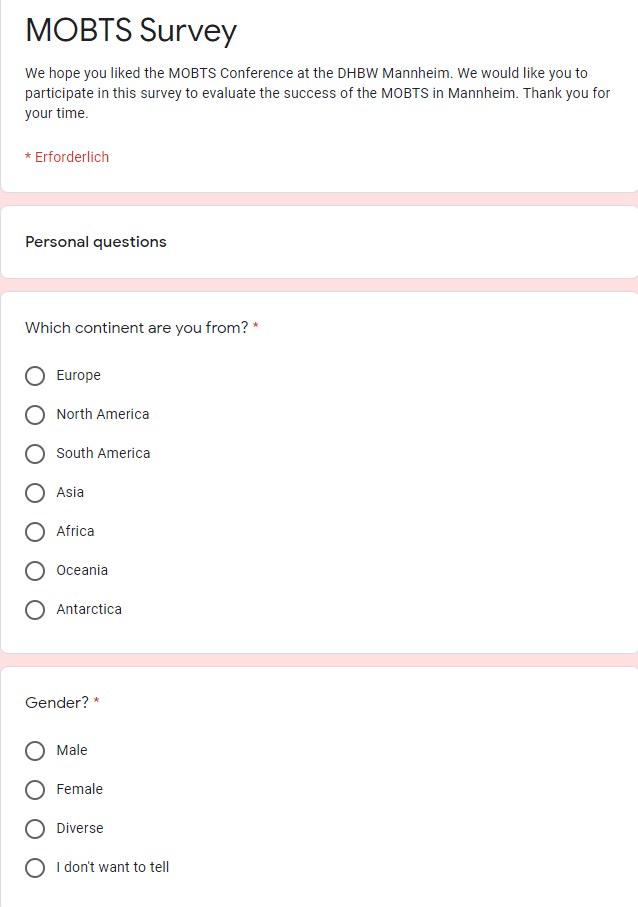
\includegraphics[width=10 cm]{img/survey1.png}
	\caption[MOBTS Umfrage]{MOBTS Umfrage Teil 1}
	\label{fig:survey1}
\end{figure}

\begin{figure}[h]
	\centering
	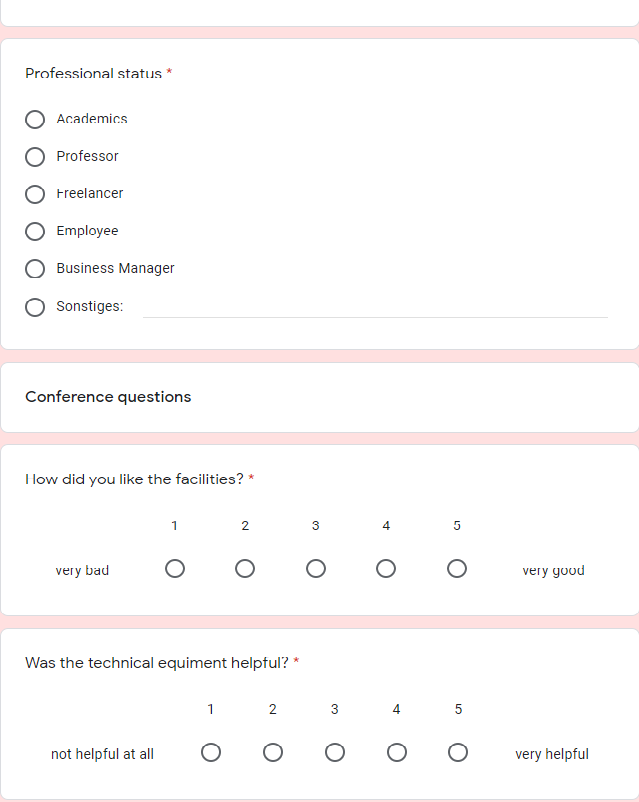
\includegraphics[width=10 cm]{img/survey2.png}
	\caption[MOBTS Umfrage]{MOBTS Umfrage Teil 2}
	\label{fig:survey2}
\end{figure}

\begin{figure}[h]
	\centering
	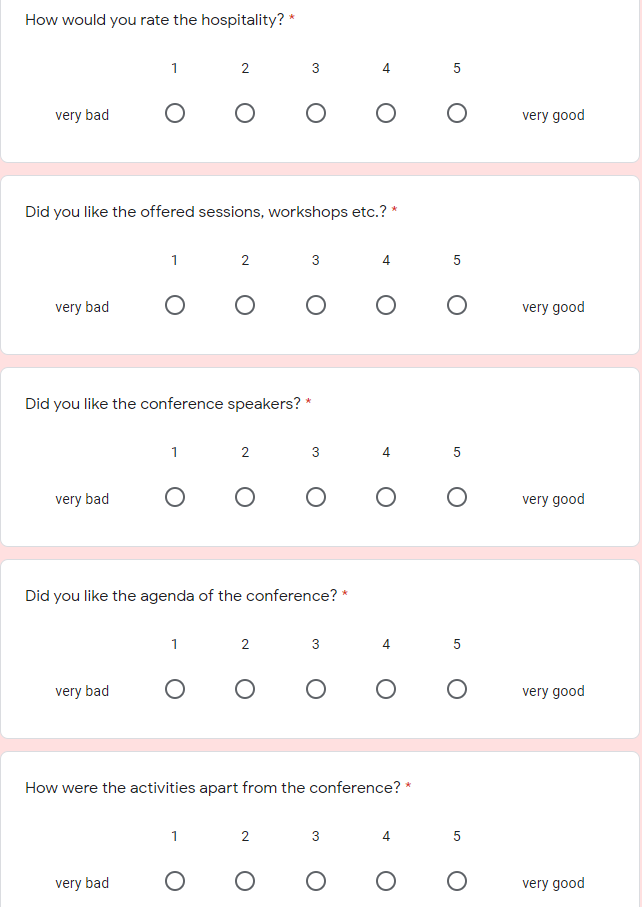
\includegraphics[width=10 cm]{img/survey3.png}
	\caption[MOBTS Umfrage]{MOBTS Umfrage Teil 3}
	\label{fig:survey3}
\end{figure}

\begin{figure}[h]
	\centering
	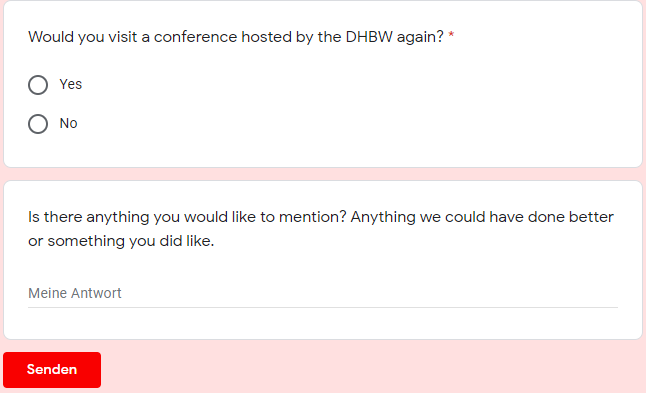
\includegraphics[width=10 cm]{img/survey4.png}
	\caption[MOBTS Umfrage]{MOBTS Umfrage Teil 4}
	\label{fig:survey4}
\end{figure}

\chapter{Catering-Angebot}
\label{app:angebot}

%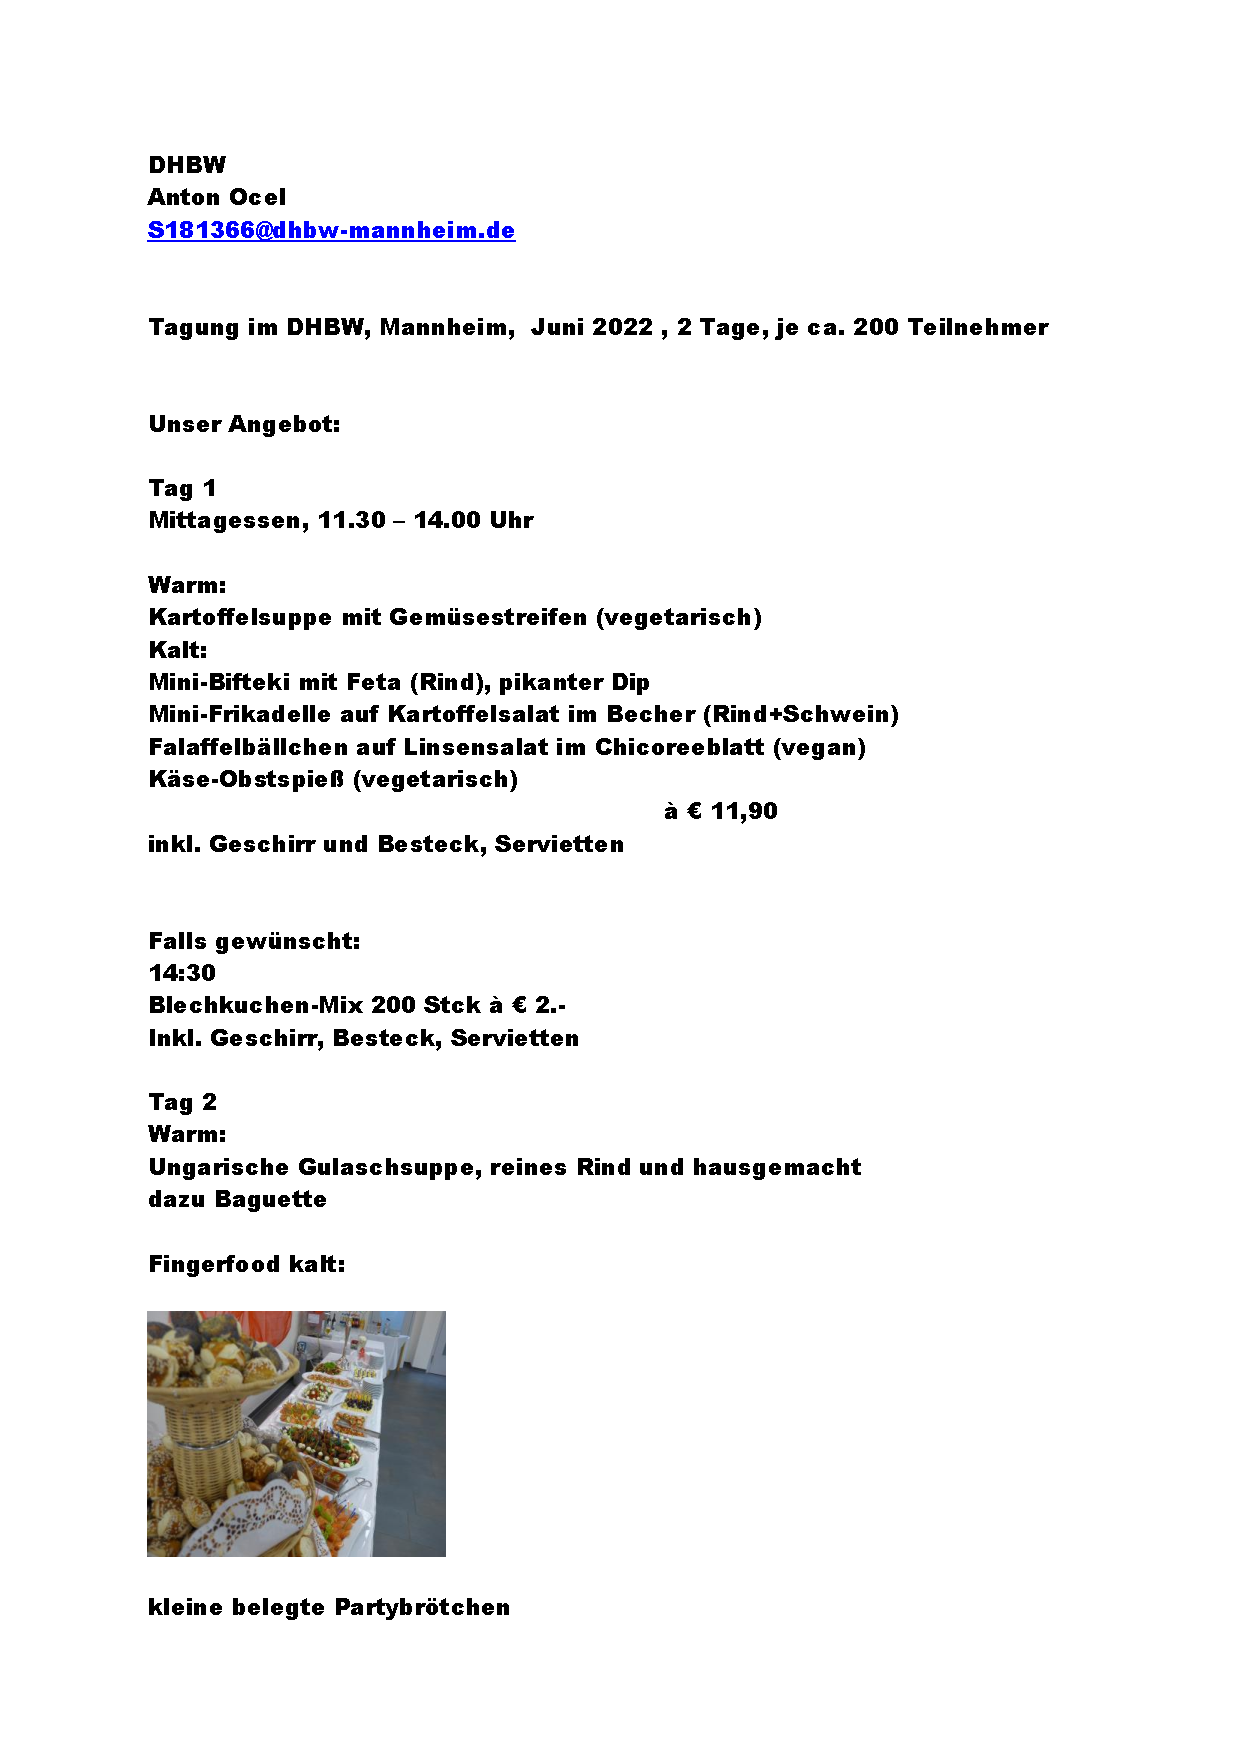
\includepdf[pages=1]{DHBWOcel2x200p22.pdf}



% Ehrenwörtliche Erklärung ewerkl.tex einziehen
% !TEX root =  master.tex

\clearpage
\chapter*{Ehrenwörtliche Erklärung}

% Wird die folgende Zeile auskommentiert, erscheint die ehrenwörtliche
% Erklärung im Inhaltsverzeichnis.

% \addcontentsline{toc}{chapter}{Ehrenwörtliche Erklärung}
Ich versichere hiermit, dass ich die vorliegende Arbeit
 mit dem Thema: \textit{\DerTitelDerArbeit} selbstständig verfasst und keine anderen als die angegebenen Quellen und
Hilfsmittel benutzt habe. Ich versichere zudem,
dass die eingereichte elektronische Fassung mit der gedruckten Fassung übereinstimmt.

\vspace{3cm}
Ort, Datum \hfill \DerAutorDerArbeit



\end{document}